\documentclass{beamer}

\setbeamertemplate{navigation symbols}{}%Double number of navigation symbols
\usepackage[utf8]{inputenc}
\usepackage{wrapfig}

\title{Summer projects at PPE}
\author{M.Kawalec \\ D.Mallows}
\setbeamercovered{transparent=25}
\date{\today}
\usetheme{default}

\begin{document}
  \frame{\titlepage 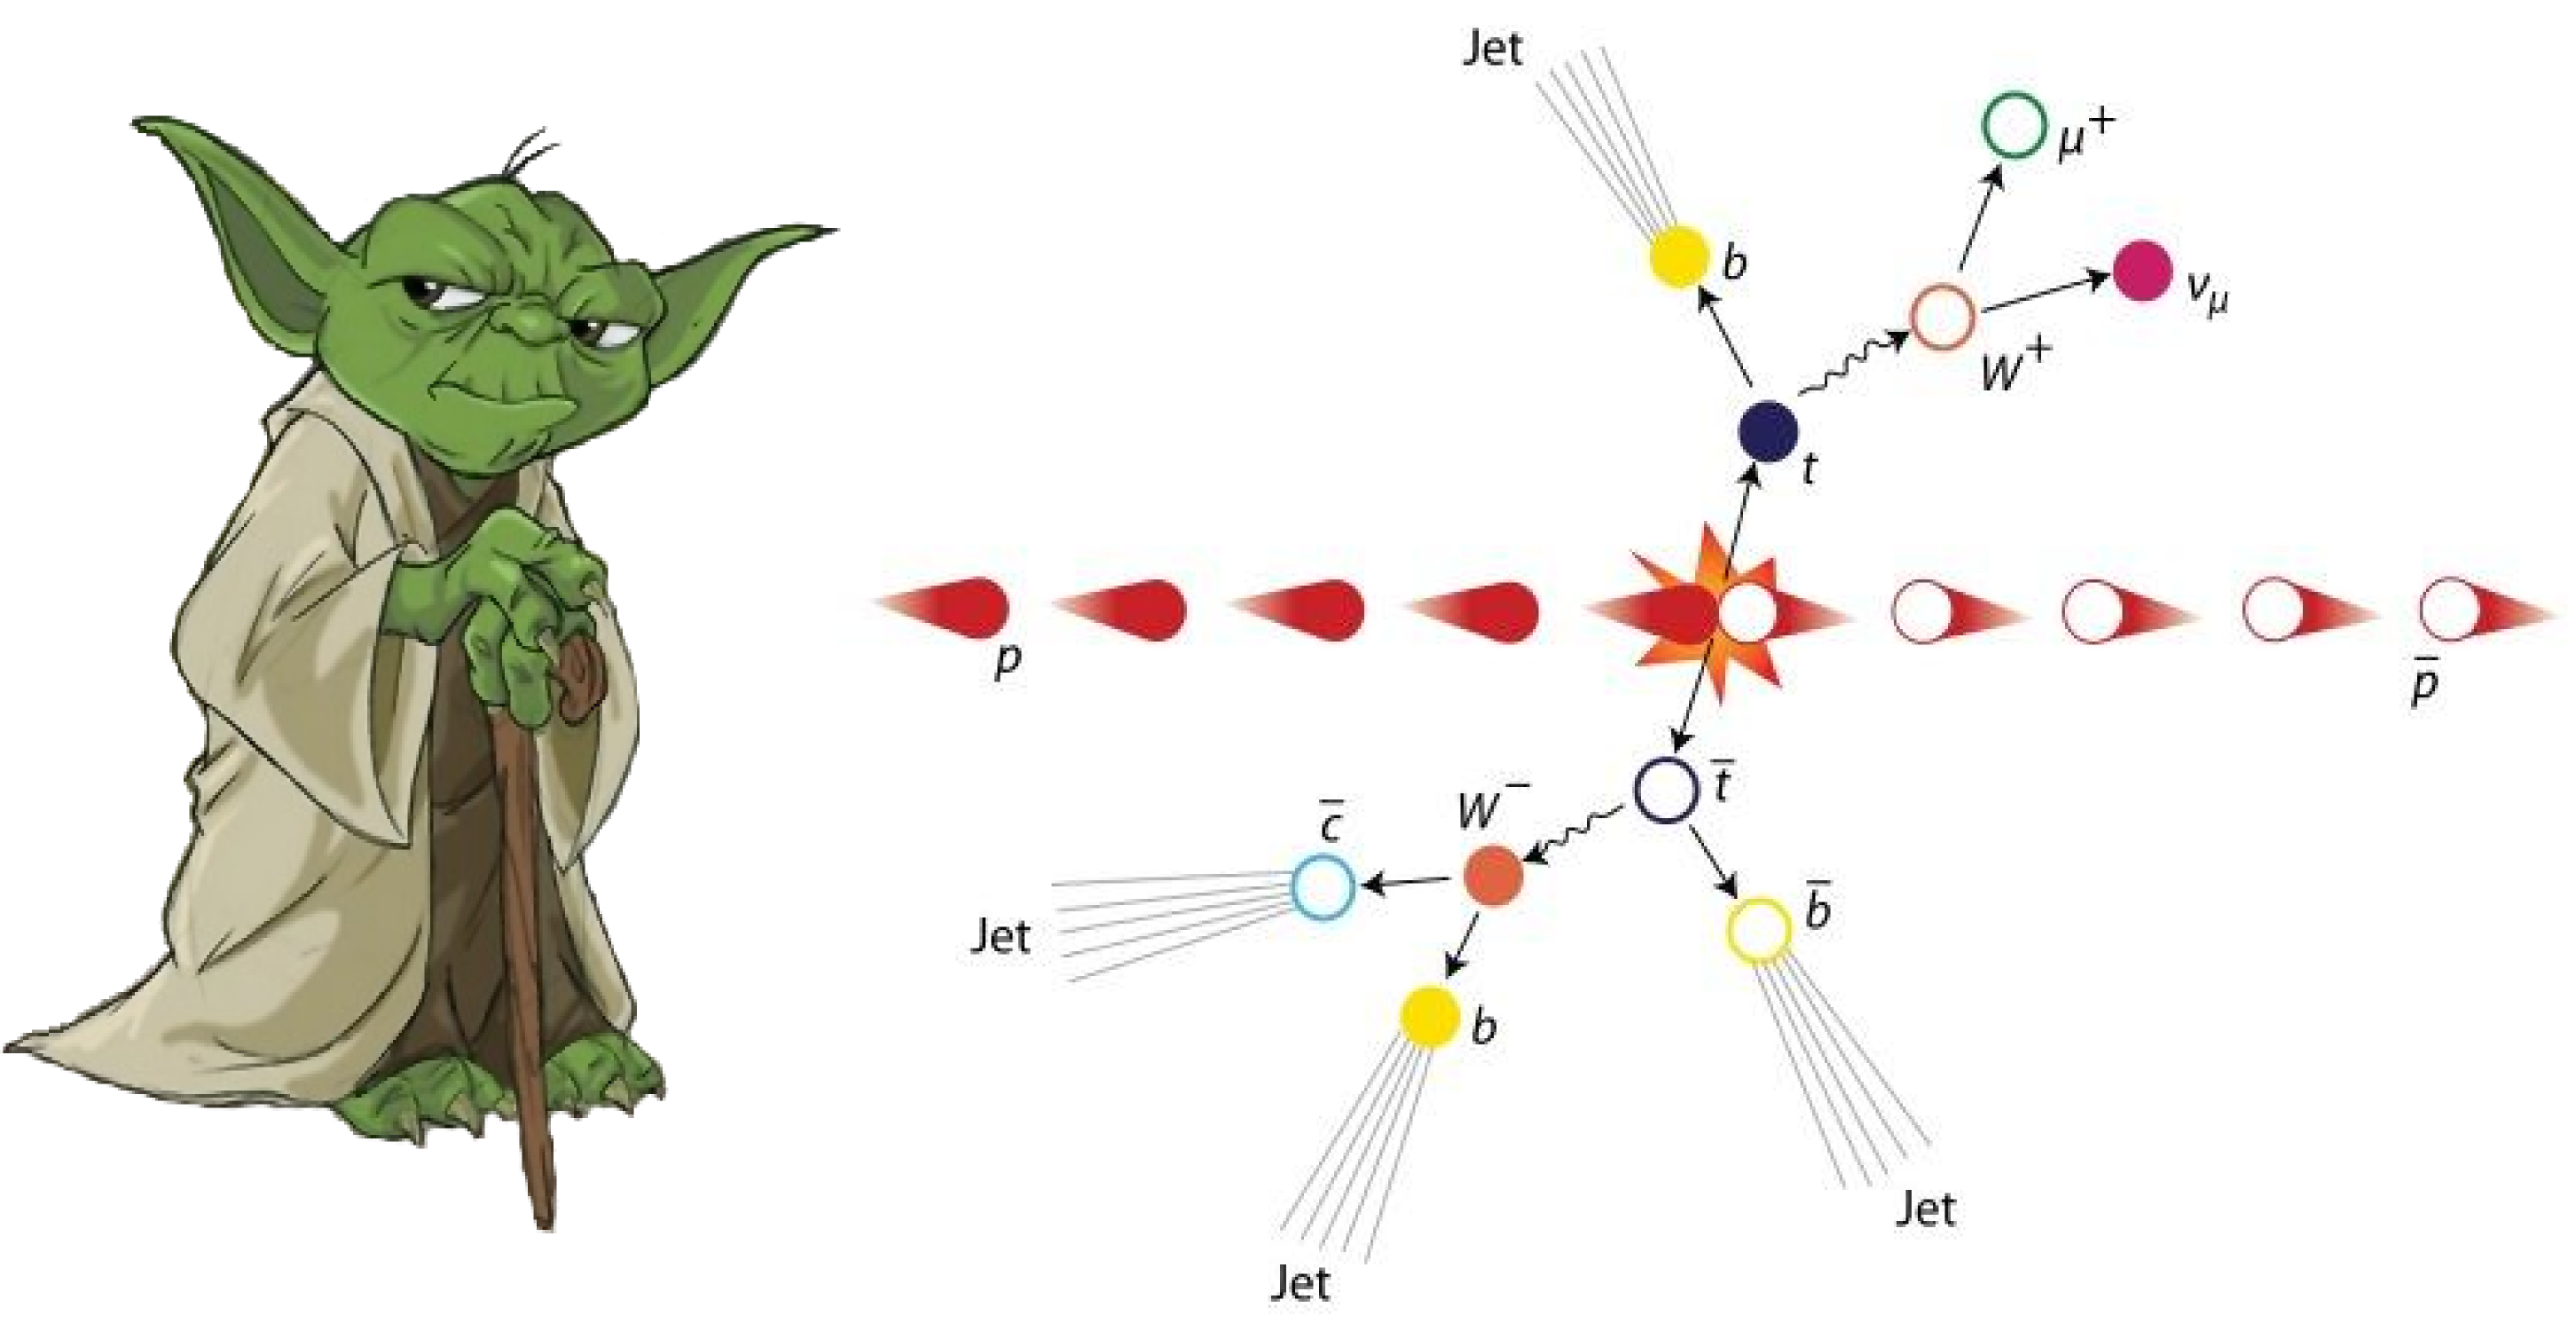
\includegraphics[height=0.4\textheight]{logos.png}}
  
%  \begin{frame}
%    \frametitle{Table of Contents}
%    \tableofcontents
%  \end{frame}

% I have said 'thou shalt not maketh anotherth fileth, we shalt useth the sameth oneth'
  
  \begin{frame}{What is YODA?}
  \begin{wrapfigure}{r}{0.5\textwidth}
  \begin{center}
    
\includegraphics[width=0.48\textwidth]{yoda-logo}
  \end{center}
  \end{wrapfigure}
  YODA is a small set of data analysis (specifically histogramming) classes being developed by MCnet members as a lightweight common system for MC event generator validation analyses. 
  \end{frame}

  \begin{frame}{YODA capabilities}
    \begin{itemize}
      \item Fully transparent and on-line bin management
      \item Efficient algorithms used under the hood
      \item Bin validation included
      \item Concise and modular codebase
      \item Python bindings 
      \item Easily extendable with new classes
    \end{itemize}
    
\includegraphics[width=0.28\textwidth]{yoda-logo}
  \end{frame}

  \begin{frame}
      \frametitle{fill() operations \ \ \ \ \ \ \ \ \ \ \ \ \ \ \ \ \ \ \ \ \ \ \ \ \ \ \ \ \ \ \ \   
\includegraphics[width=0.05\textwidth]{yoda-logo}}
      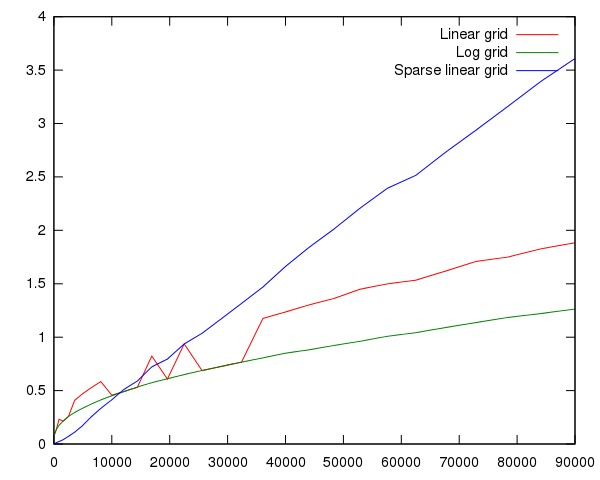
\includegraphics[height=0.89\textheight]{1.jpg}
  \end{frame}

  \begin{frame}
    \frametitle{add/rem operations \ \ \ \ \ \ \ \ \ \ \ \ \ \ \ \ \ \ \ \ \ \ \ \ \ \ \ \ \ \ \ \   
\includegraphics[width=0.05\textwidth]{yoda-logo}}
    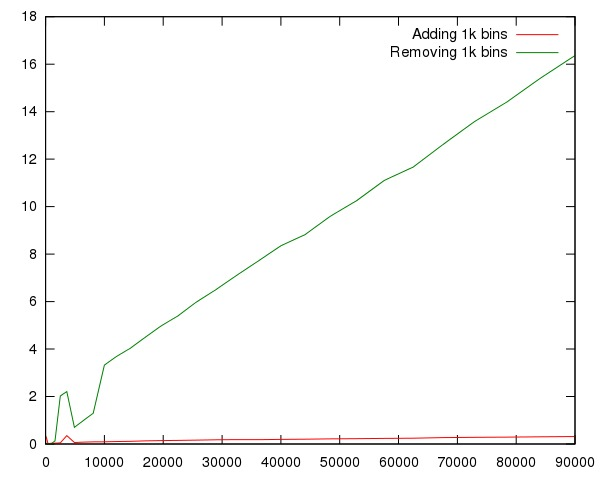
\includegraphics[height=0.89\textheight]{2.jpg}
  \end{frame}

  \begin{frame}
    \frametitle{rebin() all bins \ \ \ \ \ \ \ \ \ \ \ \ \ \ \ \ \ \ \ \ \ \ \ \ \ \ \ \ \ \ \ \   
\includegraphics[width=0.05\textwidth]{yoda-logo}}
    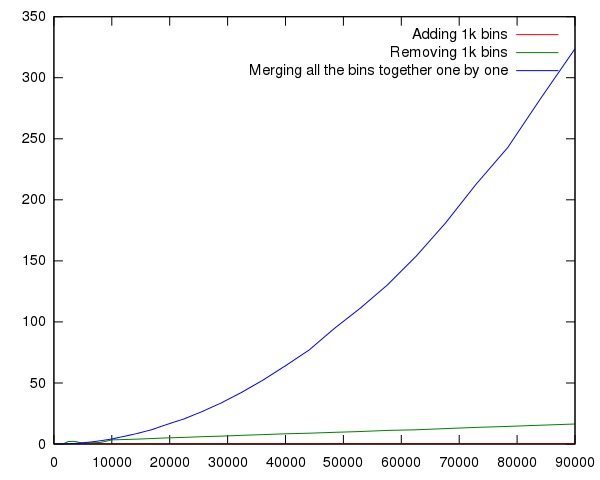
\includegraphics[height=0.89\textheight]{2a.jpg}
  \end{frame}

  \begin{frame}
    \frametitle{Top production route \ \ \ \ \ \ \ \ \ \ \ \ \ \ \ \ \ \ \ \ \ \ \ \ \ \ \ \ \ \ \ \   
\includegraphics[width=0.05\textwidth]{yoda-logo}}
    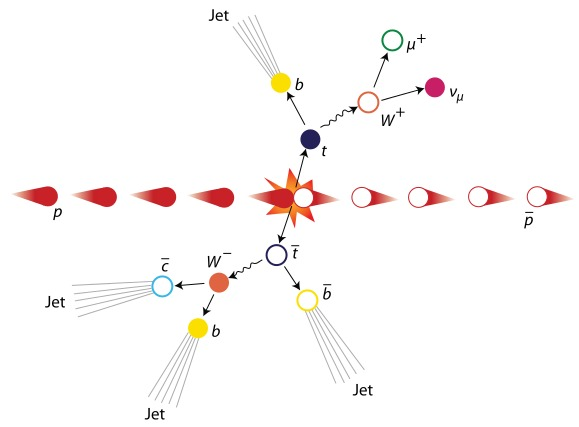
\includegraphics[height=0.89\textheight]{ttbar.jpg}
  \end{frame}

  \begin{frame}
    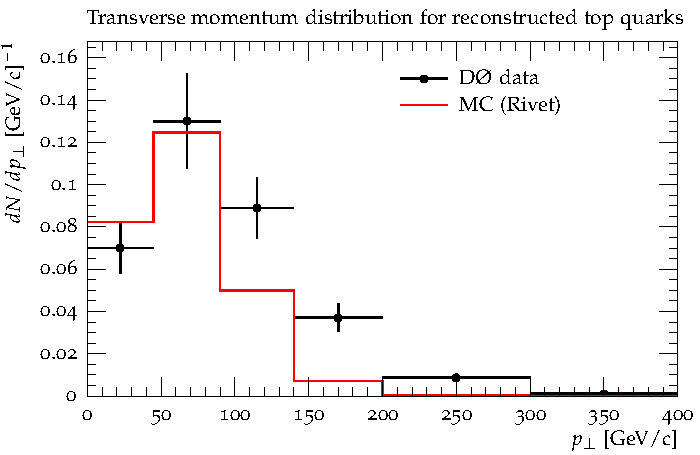
\includegraphics[width=\textwidth]{top_paper}
  \end{frame}

  \begin{frame}{Top reconstruction - naive approach}
    \begin{itemize}
      \item One charged lepton
      \item Jet-finding algorithm
      \item Tag jets containing hadronised b-particles 
      \item Reconstruct hadronically decaying W's mass from non b-tagged jets
      \item Place cuts on W mass (instead of weighting function)
      \item Reconstruct $t$, $\bar{t}$ pair
    \end{itemize}
    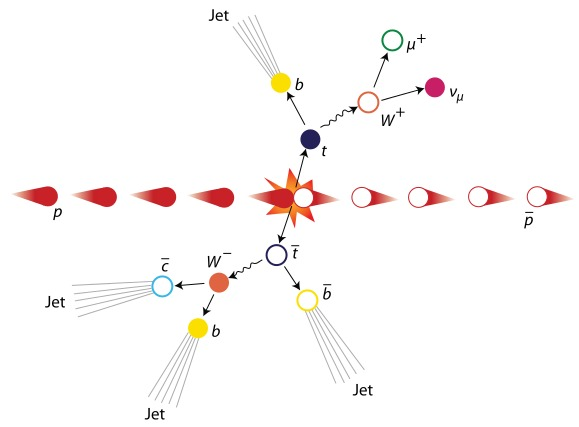
\includegraphics[height=0.4\textheight]{ttbar.jpg}
  \end{frame}

  \begin{frame}{Top reconstruction - improvements}
    \begin{itemize}
      \item Reconstruct leptonically decaying W as well
      \item Select combinations of l-jets that minimise difference in W-masses
      \item Choose t, tbar pair that minimises difference between t, tbar masses
      \item Change Pythia parameters!
    \end{itemize}
    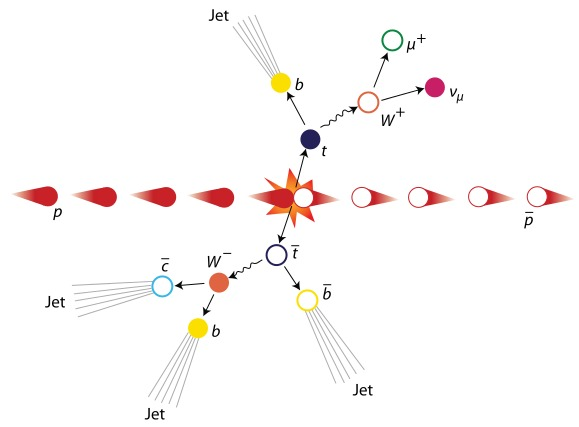
\includegraphics[height=0.4\textheight]{ttbar.jpg}
  \end{frame}

  \begin{frame}
    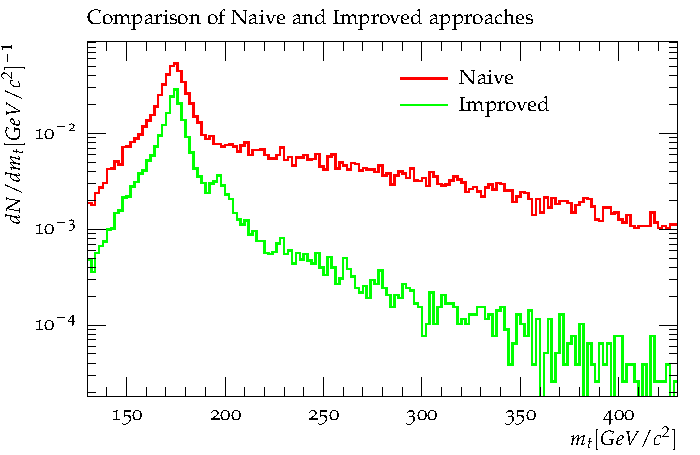
\includegraphics[width=\textwidth]{comparison}
  \end{frame}
	
  \begin{frame}{Plotting}
    \begin{itemize}
      \item Rivet uses make-plots
      \item Produces excellent plots
      \item Outgrown initial goals
    \end{itemize}
  \end{frame}
  \begin{frame}
    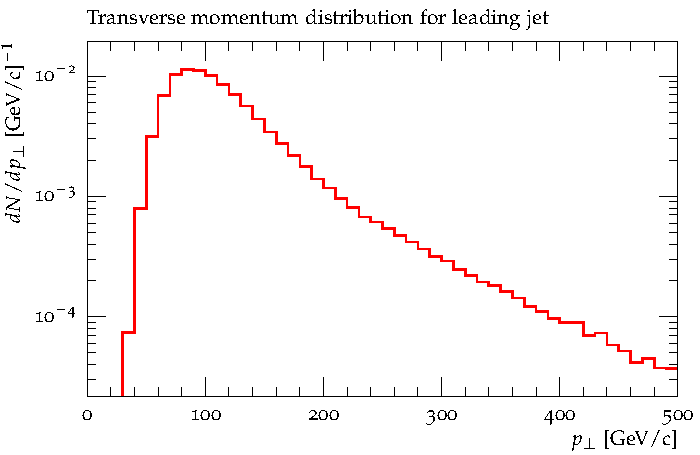
\includegraphics[width=\textwidth]{makeplots}
  \end{frame}

  \begin{frame}{The ideal scientific plotting package}
    \begin{itemize}
      \item \LaTeX\ -- use what you already use
      \item Preview -- see changes as they happen
      \item Aimed at Physical Sciences
      \item Clear focus on graphics for print, not screen
      \item Simplicity over esoteric features
      \item Sane defaults
    \end{itemize}
  \end{frame}

  \begin{frame}{The not-so-ideal scientific plotting package}
    
    \begin{itemize}
      \item A concise Python drawing library which uses \TeX\ for text placement.
      \item Output as \LaTeX, PDF, PNG, SVG and on-screen preview
      \item Plotting library with heirarchical parameters
      \item First release {\em imminent}, along with thin wrapper for YODA
    \end{itemize}
  \end{frame}
  \begin{frame}
    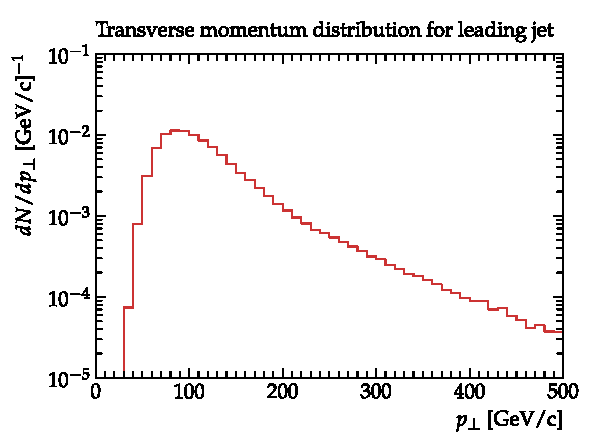
\includegraphics[width=\textwidth]{daveplot}
  \end{frame}

\end{document}
